\documentclass[margin=3mm]{standalone}
\usepackage[american]{circuitikz} % Usamos el estilo americano/estándar de componentes

\begin{document}
	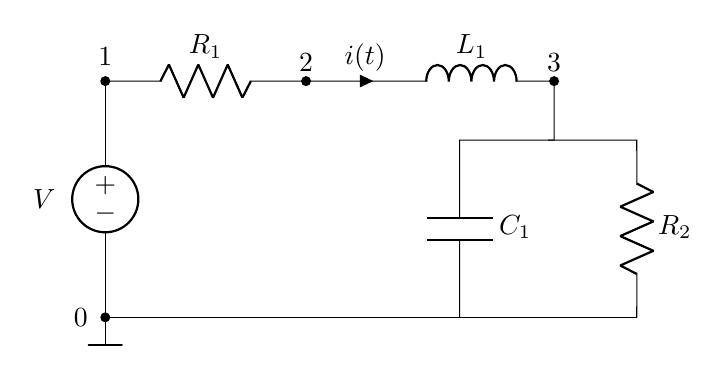
\begin{tikzpicture}[scale=1.5]
		% Nodo de referencia (Tierra) en la parte inferior
		\draw (0,0) node[rground] (ground) {};		
		% Rama de la fuente V1 (Nodo 0 a Nodo 1)
		\draw (0,0) to[V, invert, v=$V$] (0,2) 
		  to[short, -*] ++(0,0)node [above=0.5ex]{$1$};		
		% Rama serie superior: R1 (1 a 2) y L1 (2 a 3)
		\draw (0,2) to[R, l=$R_1$] (1.7,2) to[short, -*] ++(0,0) node[above] {2}
		to [short, i=$i(t)$] ++ (1,0)
		to[L, l=$L_1$] (3.5,2) to[short, -*] ++(0.3,0)node[above] {3}		
		% Derivación vertical para los componentes en paralelo en el Nodo 3		% Rama en paralelo 1: R2 (Nodo 3 a 0)
to ++(0,-0.5) -- (3,1.5)
to[C, l=$C_1$] (3,0) -- (3,0);		
		% Rama en paralelo 2: C1 (Nodo 3 a 0)
		\draw (3.75,1.5) -- (4.5,1.5)
		to[R, l=$R_2$] (4.5,0);		
		% Cierre de conexiones hacia la toma de tierra común
		\draw (4.5,0) -- (0,0)to[short, -*] ++(0,0) node[left=1mm] {0};		
	\end{tikzpicture}
\end{document}
